\section{Results} \label{results}

\subsection{Models} \label{results:models}
Multiple models were used to evaluate the implemented methods in section \ref{implementation}. The model with the largest scale is the Disney cloud \cite{DisneyCloud}. Our implementation is bound by volumes with size $4096^3$ so we use the half resolution version. Armadillo and fire from the \href{https://www.openvdb.org/download/}{OpenVDB website}. Armadillo is a model with high dimensions, but only has density values on the border of the model, which makes it completely hollow. Animation models from the \href{https://jangafx.com/software/embergen/download/free-vdb-animations/}{JangaFX website} were used, namely, Industrial Chimney Smoke. This model has many small frames, this stresses the per-frame tree size. Since we are not specifically interested the tree size, but more so in the voxel data size, we decided to only use the first n frames of the animation.

\subsection{Tree size} \label{results:tree_size}
\subsection{Block compression} \label{results:block_compression}

\begin{figure}[H]
    \centering
    %\subfloat[]{
    %    \includegraphics[width=0.45\textwidth]{}
    %}
    %\hfill
    %\subfloat[]{
    %    \includegraphics[width=0.45\textwidth]{}
    %}

    \caption{} \label{fig:implementation:compression:bc}
\end{figure}
\subsection{Clustering} \label{results:clustering}


\begin{figure}[H]
    \centering
    \subfloat[]{
        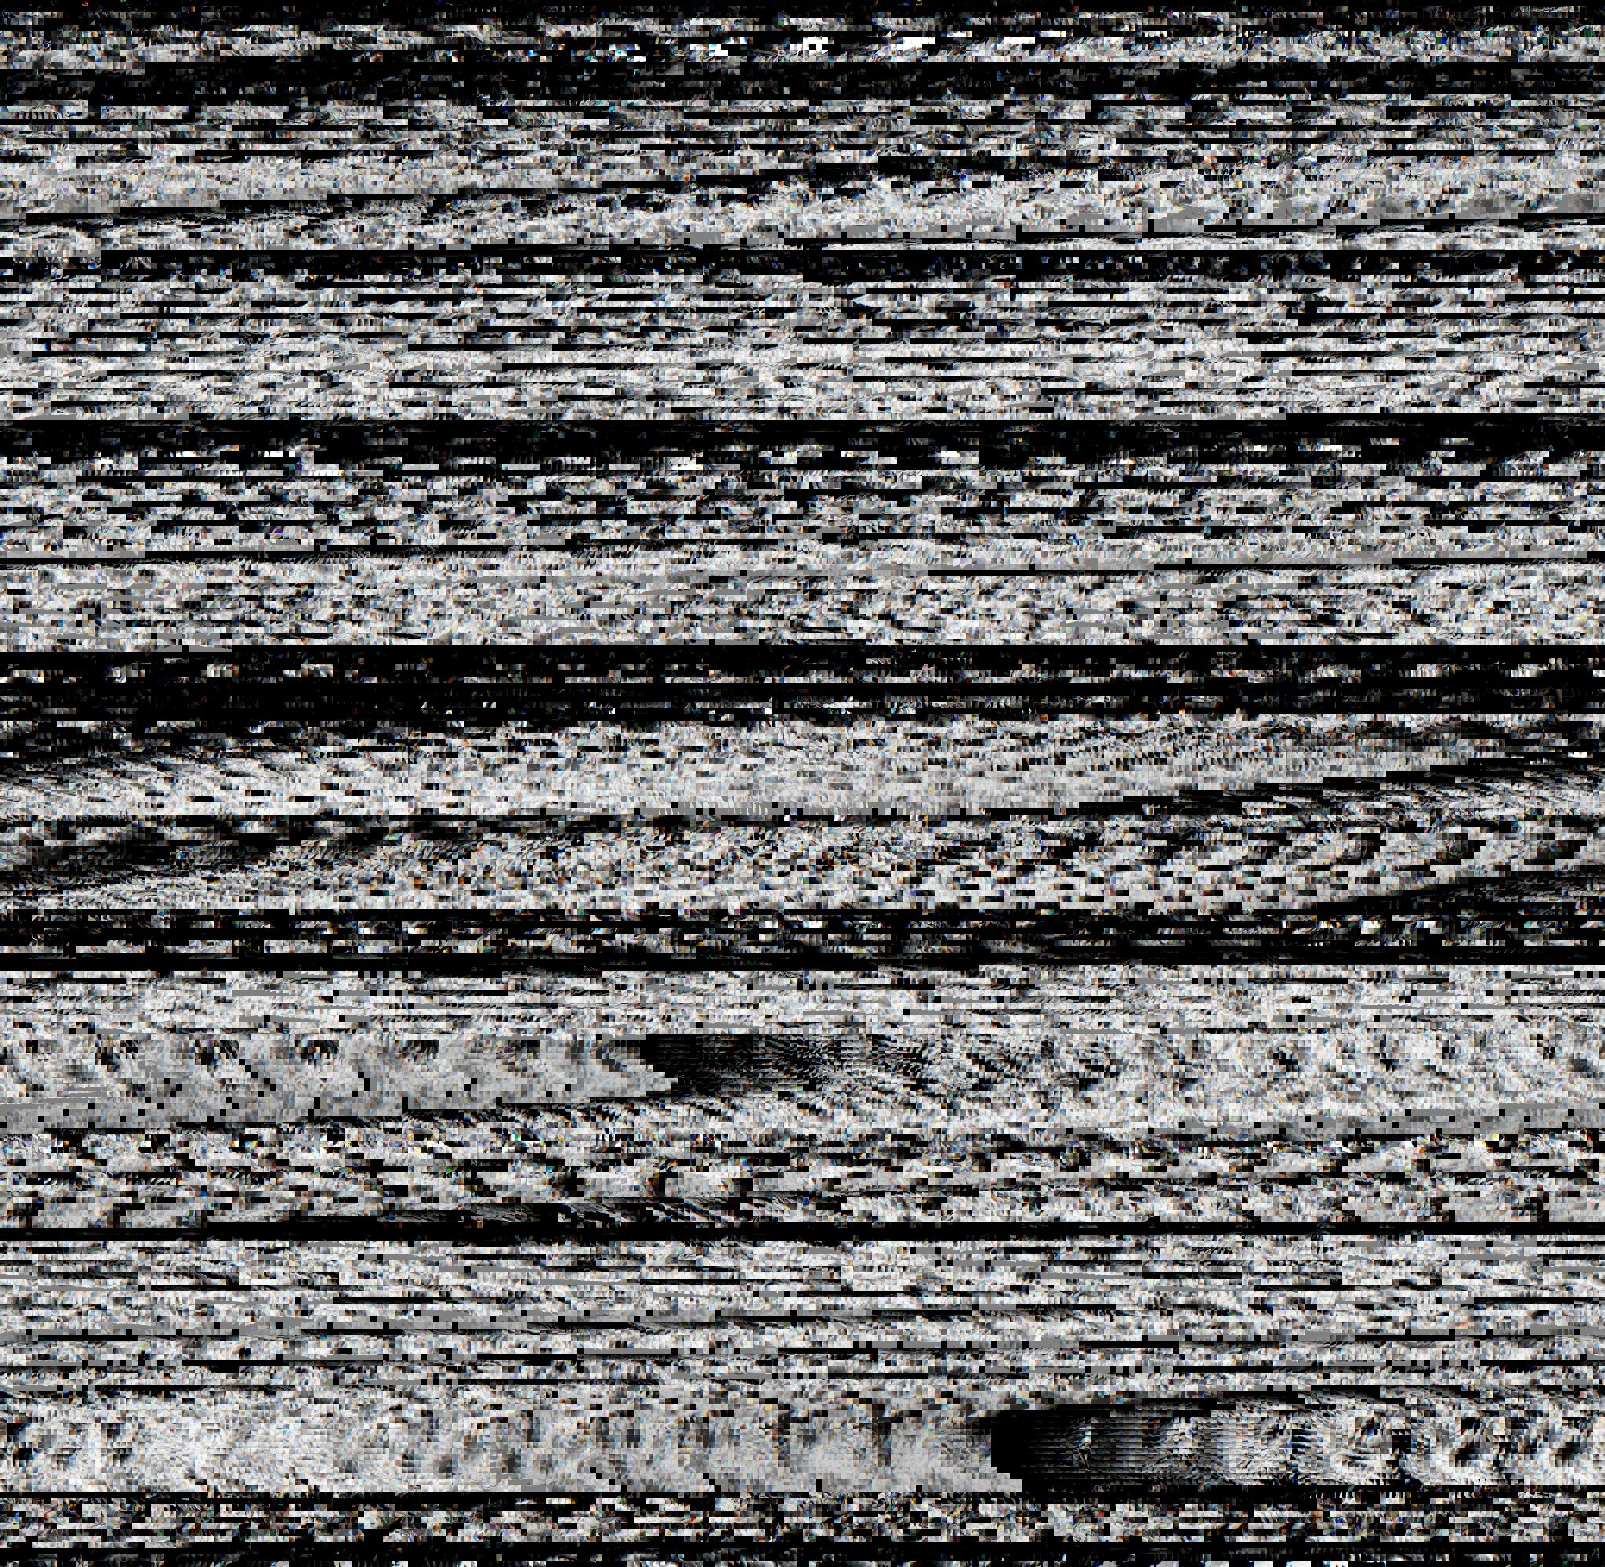
\includegraphics[width=0.45\textwidth]{figures/pre_clustered_memory.png} \label{fig:implementation:compression:pre_cluster}
    }
    \hfill
    \subfloat[]{
        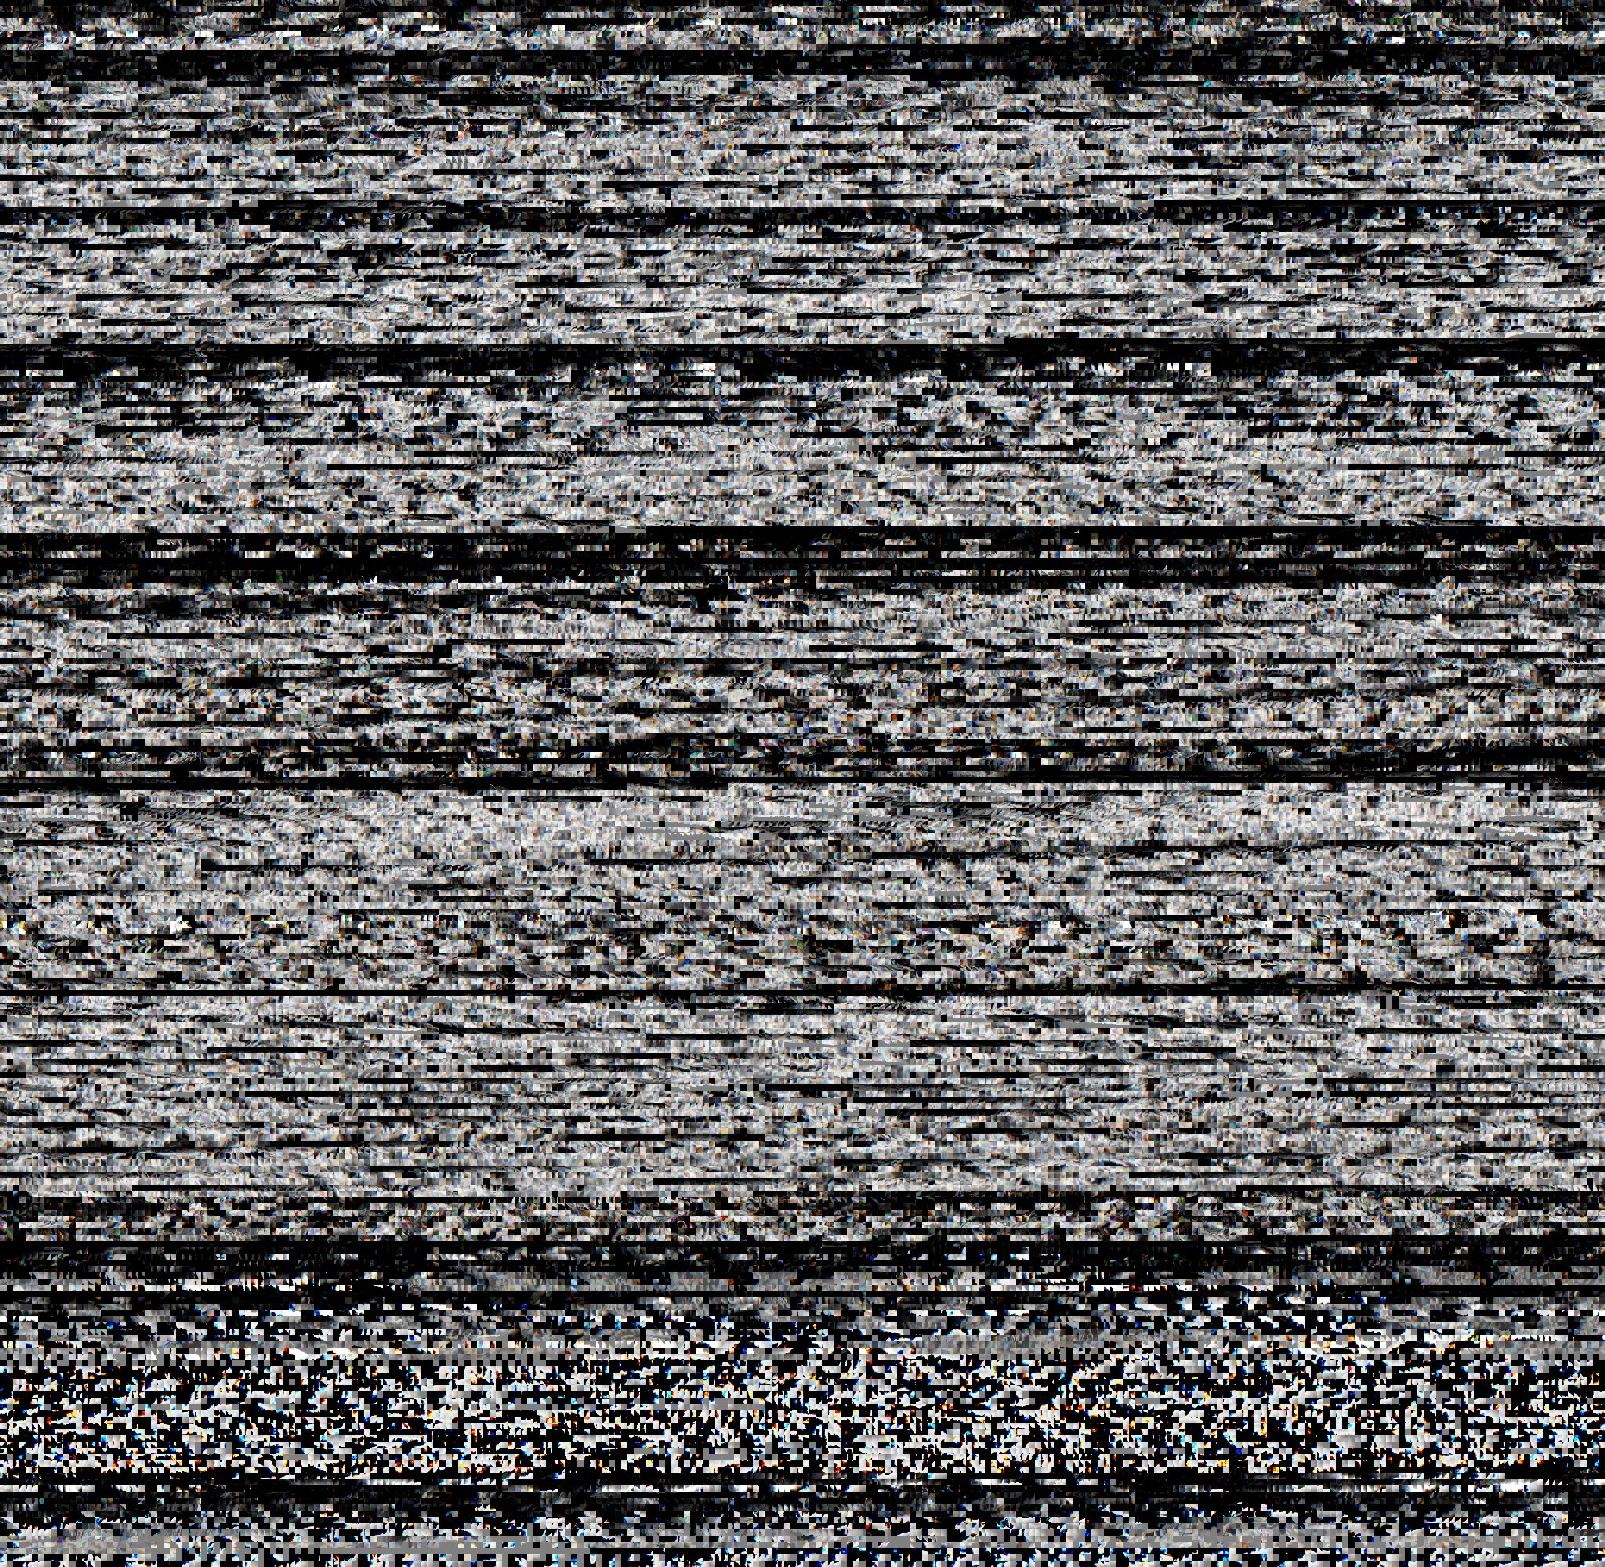
\includegraphics[width=0.45\textwidth]{figures/post_clustered_memory.png} \label{fig:implementation:compression:post_cluster}
    }
    \caption{The results of our clustering compression technique. All of these results use Bc7 encoding. Figure \ref{fig:implementation:compression:pre_cluster} shows a slice out of the voxel brick data texture on the GPU. There are visible long chains of black or otherwise greyscale slices which means that these bricks are mostly homogeneous inside that brick. In Figure \ref{fig:implementation:compression:post_cluster} we again see a slice of the voxel brick data texture, but this time after running our clustering algorithm. There are visibly fewer patches greyscale bricks when compared to figure \ref{fig:implementation:compression:pre_cluster}. This shows us that we are actually removing bricks which are homogeneous, and keeping unique nodes.} \label{fig:implementation:compression:cluster}
\end{figure}